\section[P vs NP]{Motivations to go nonparametric}

\begin{frame}{Parametric versus nonparametric}
 
\begin{block}{Parametric models}
\begin{itemize}
	\item Finite and fixed number of parameters  
	\item Number of parameters is independent of the dataset
\end{itemize}
\end{block}

\begin{block}{Nonparametric models}
	\begin{itemize}
		\item Do have parameters
		\item Can be understood as having an infinite number of  parameters 
		\item Can be understood as having a random number of  parameters
		\item Number of parameters can grow with the dataset
	\end{itemize}
\end{block}
\end{frame}



%%%%%%%%%%%%%%%%%%%%%%%%%%%%%%%%%%%%%%%%%%%%%%%%%%%%%%%%%%%%%%%%%%%%%%%%%%%%%%%%%%%%%%%%%%%%%%%%%%%%%%
\frame{\frametitle{Underlying function}
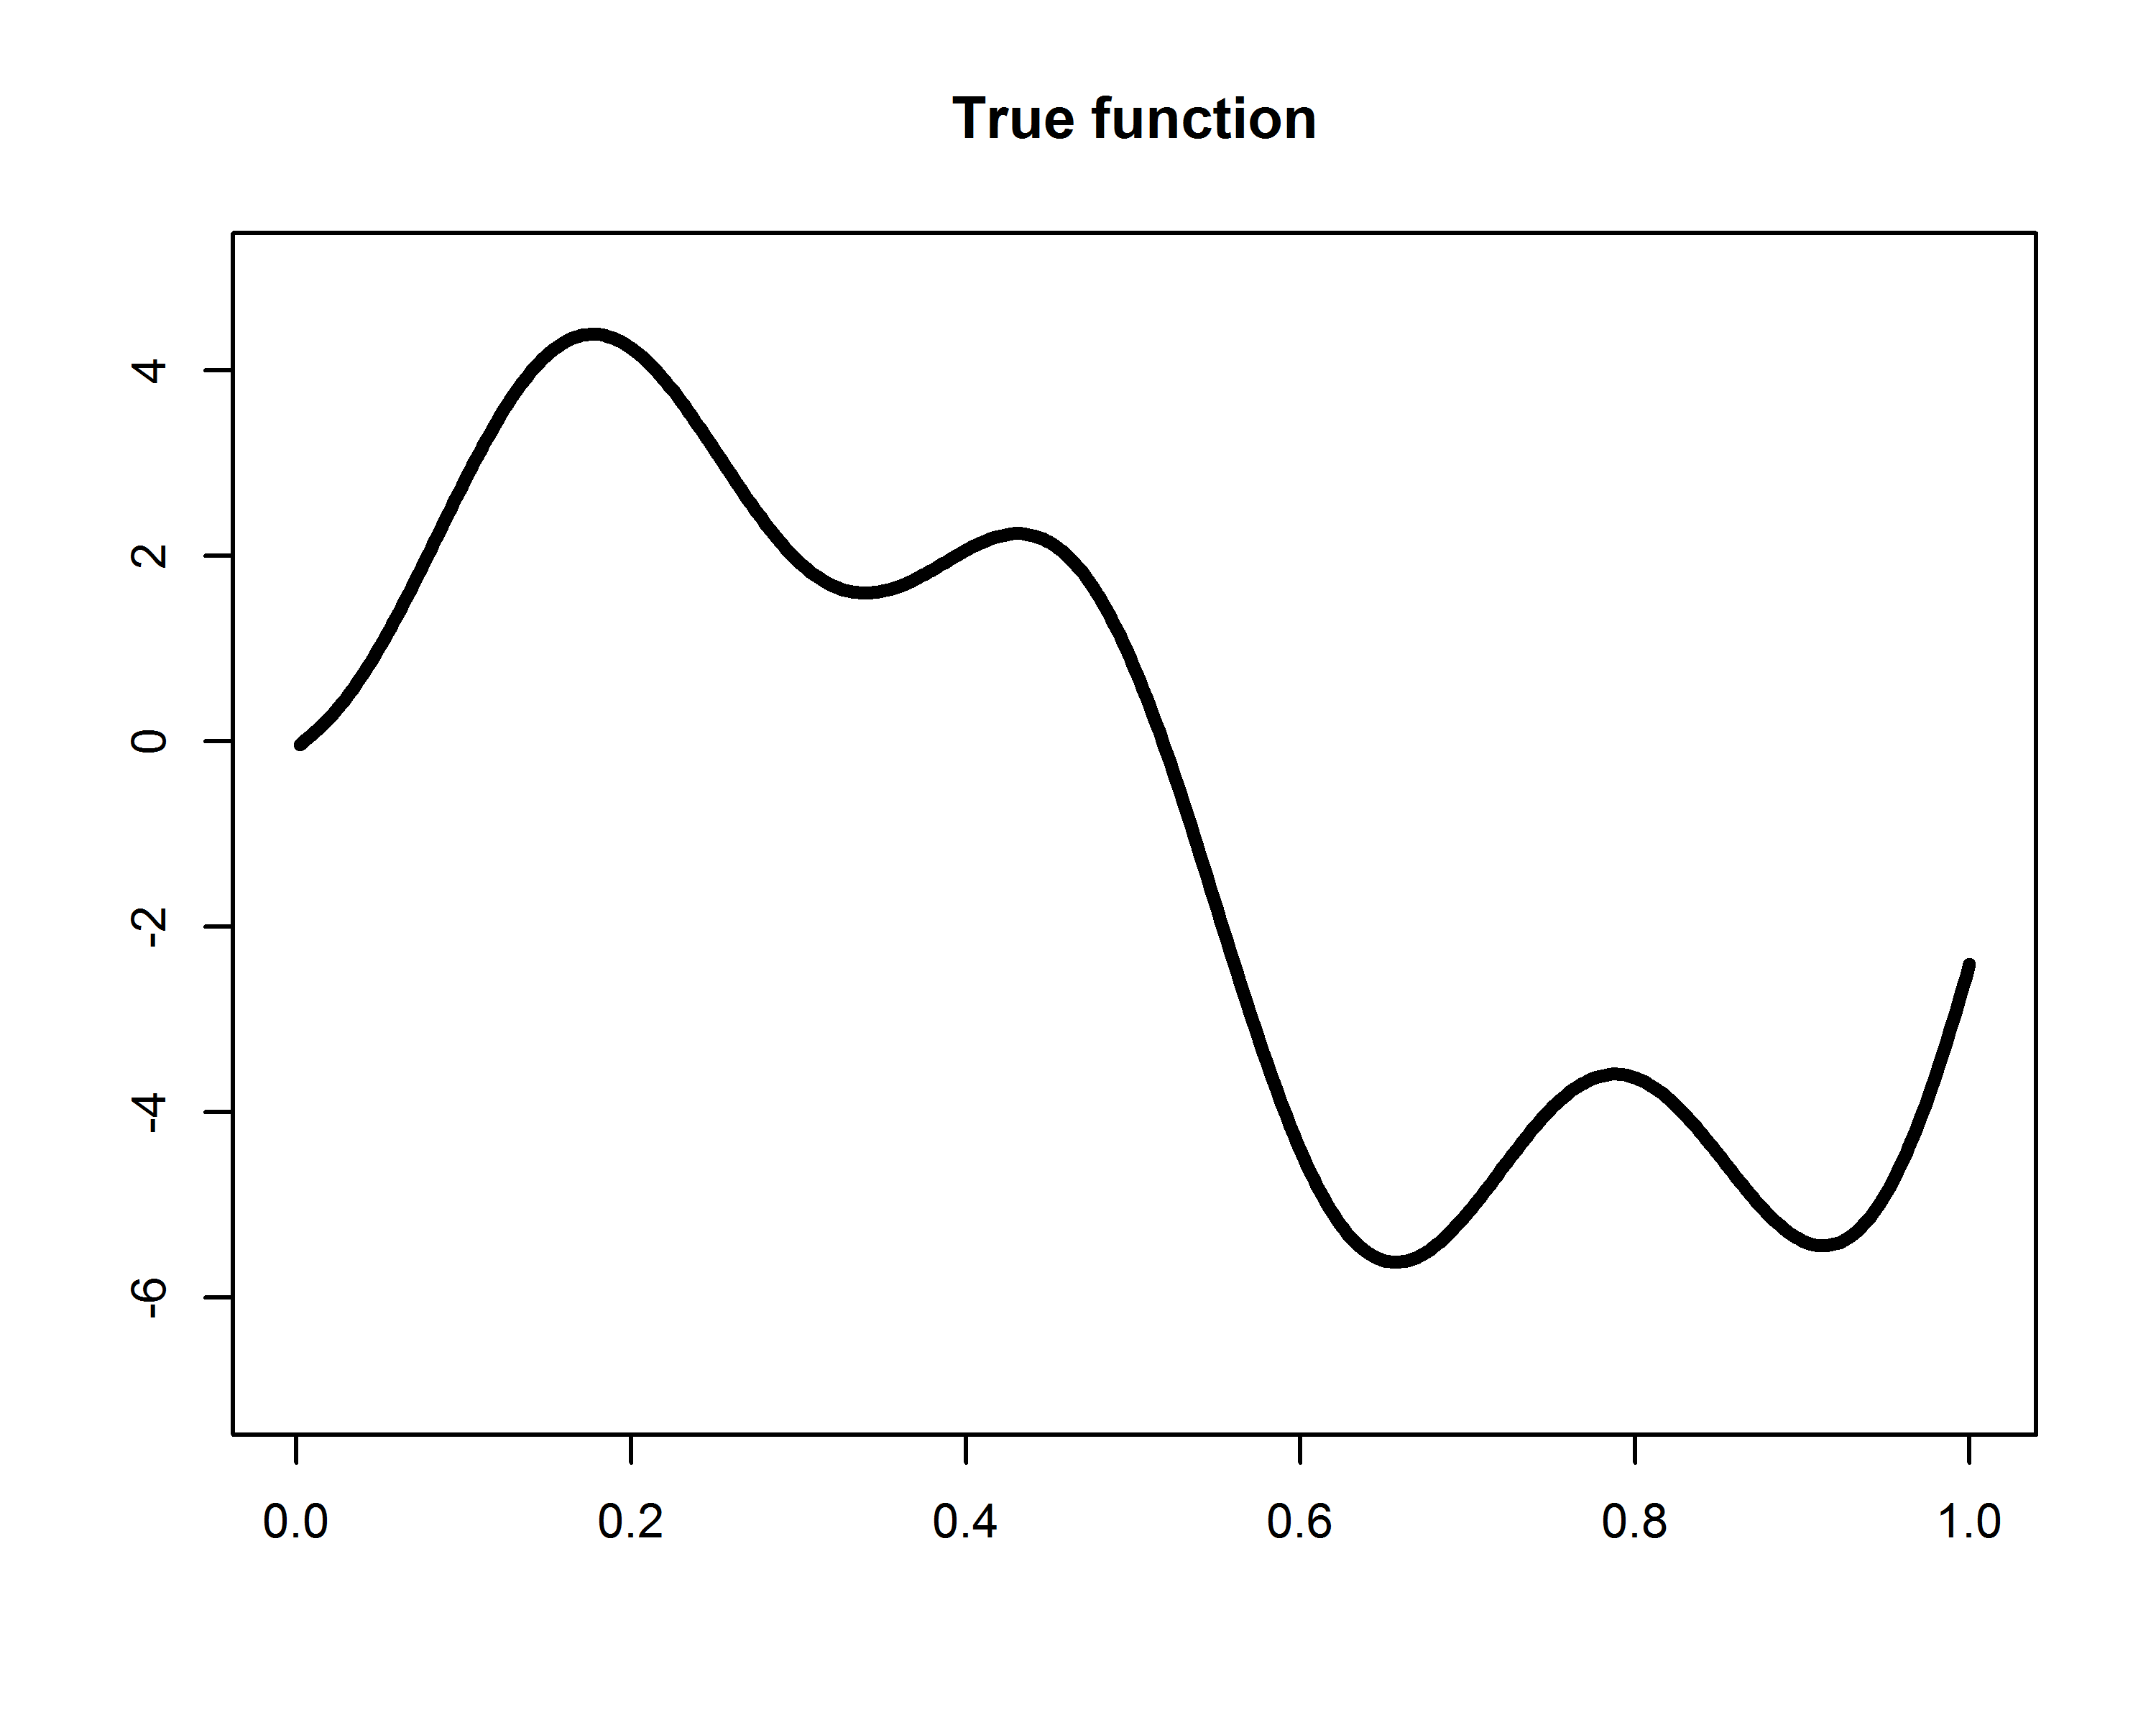
\includegraphics[width = 4in]{figures_julyan/Botond/true.png}
}


\frame{\frametitle{Data}
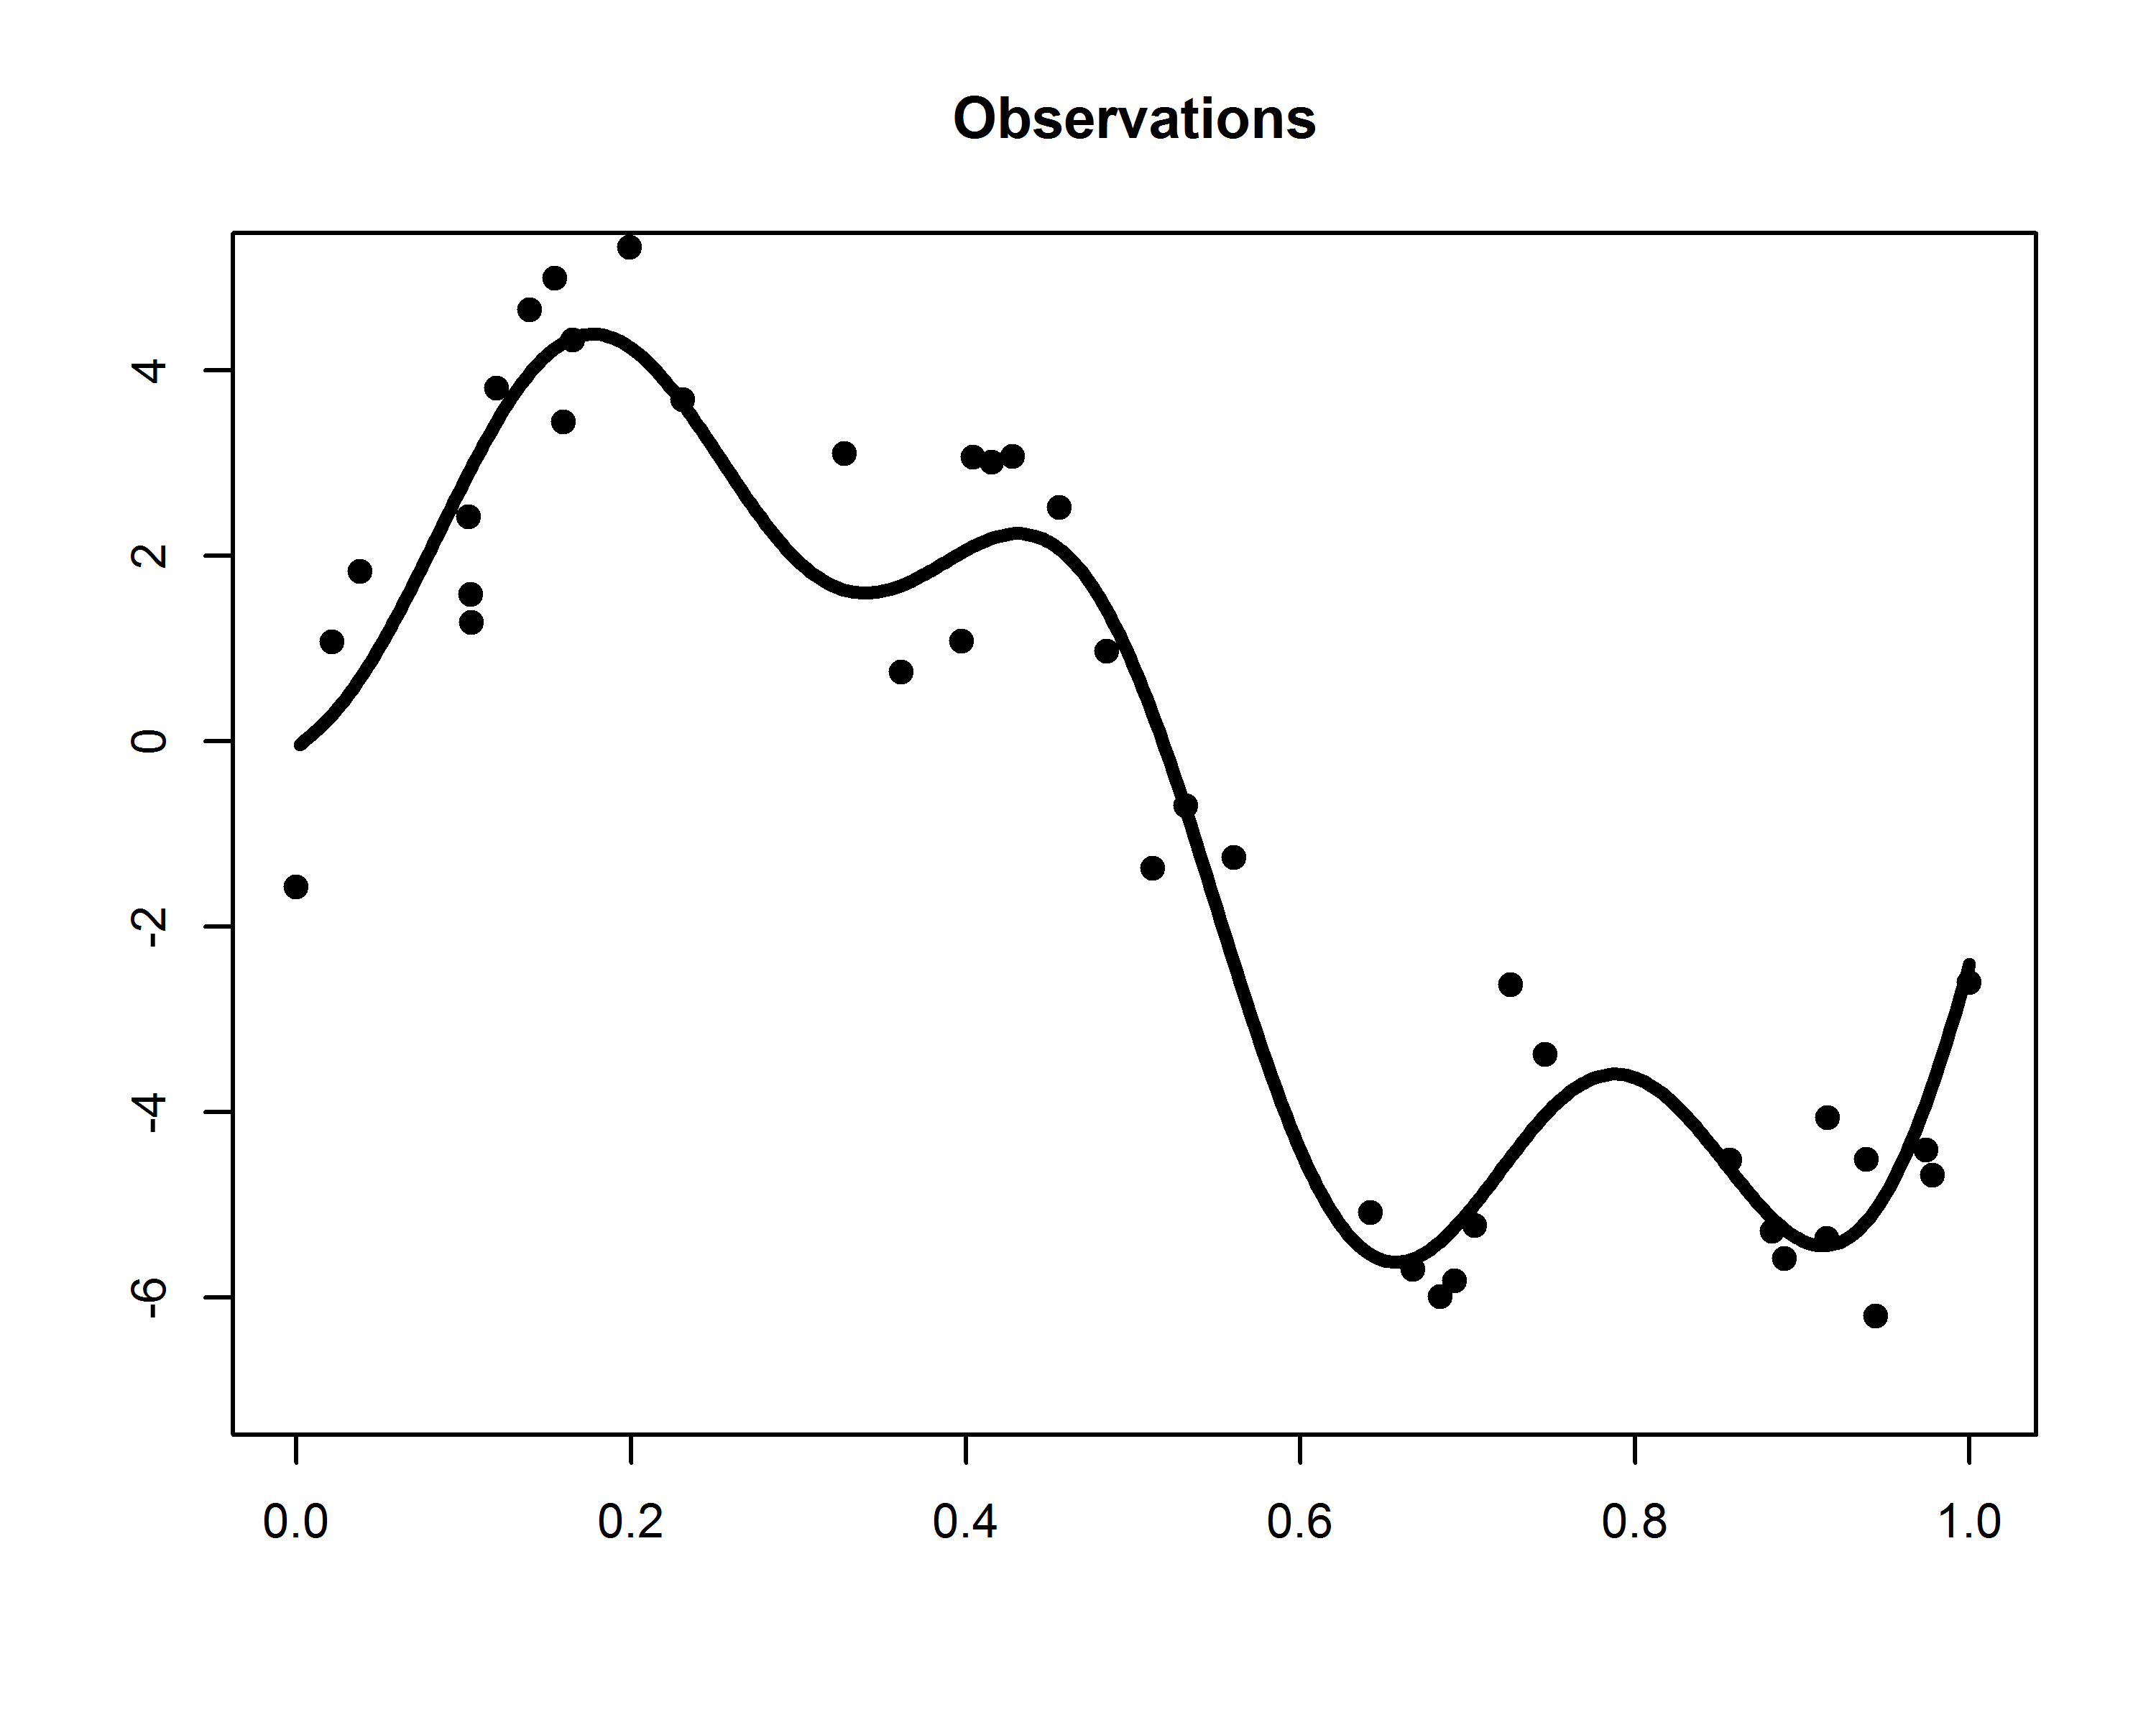
\includegraphics[width = 4in]{figures_julyan/Botond/TrueData2.png}
}


\frame{\frametitle{Parametric fitting}
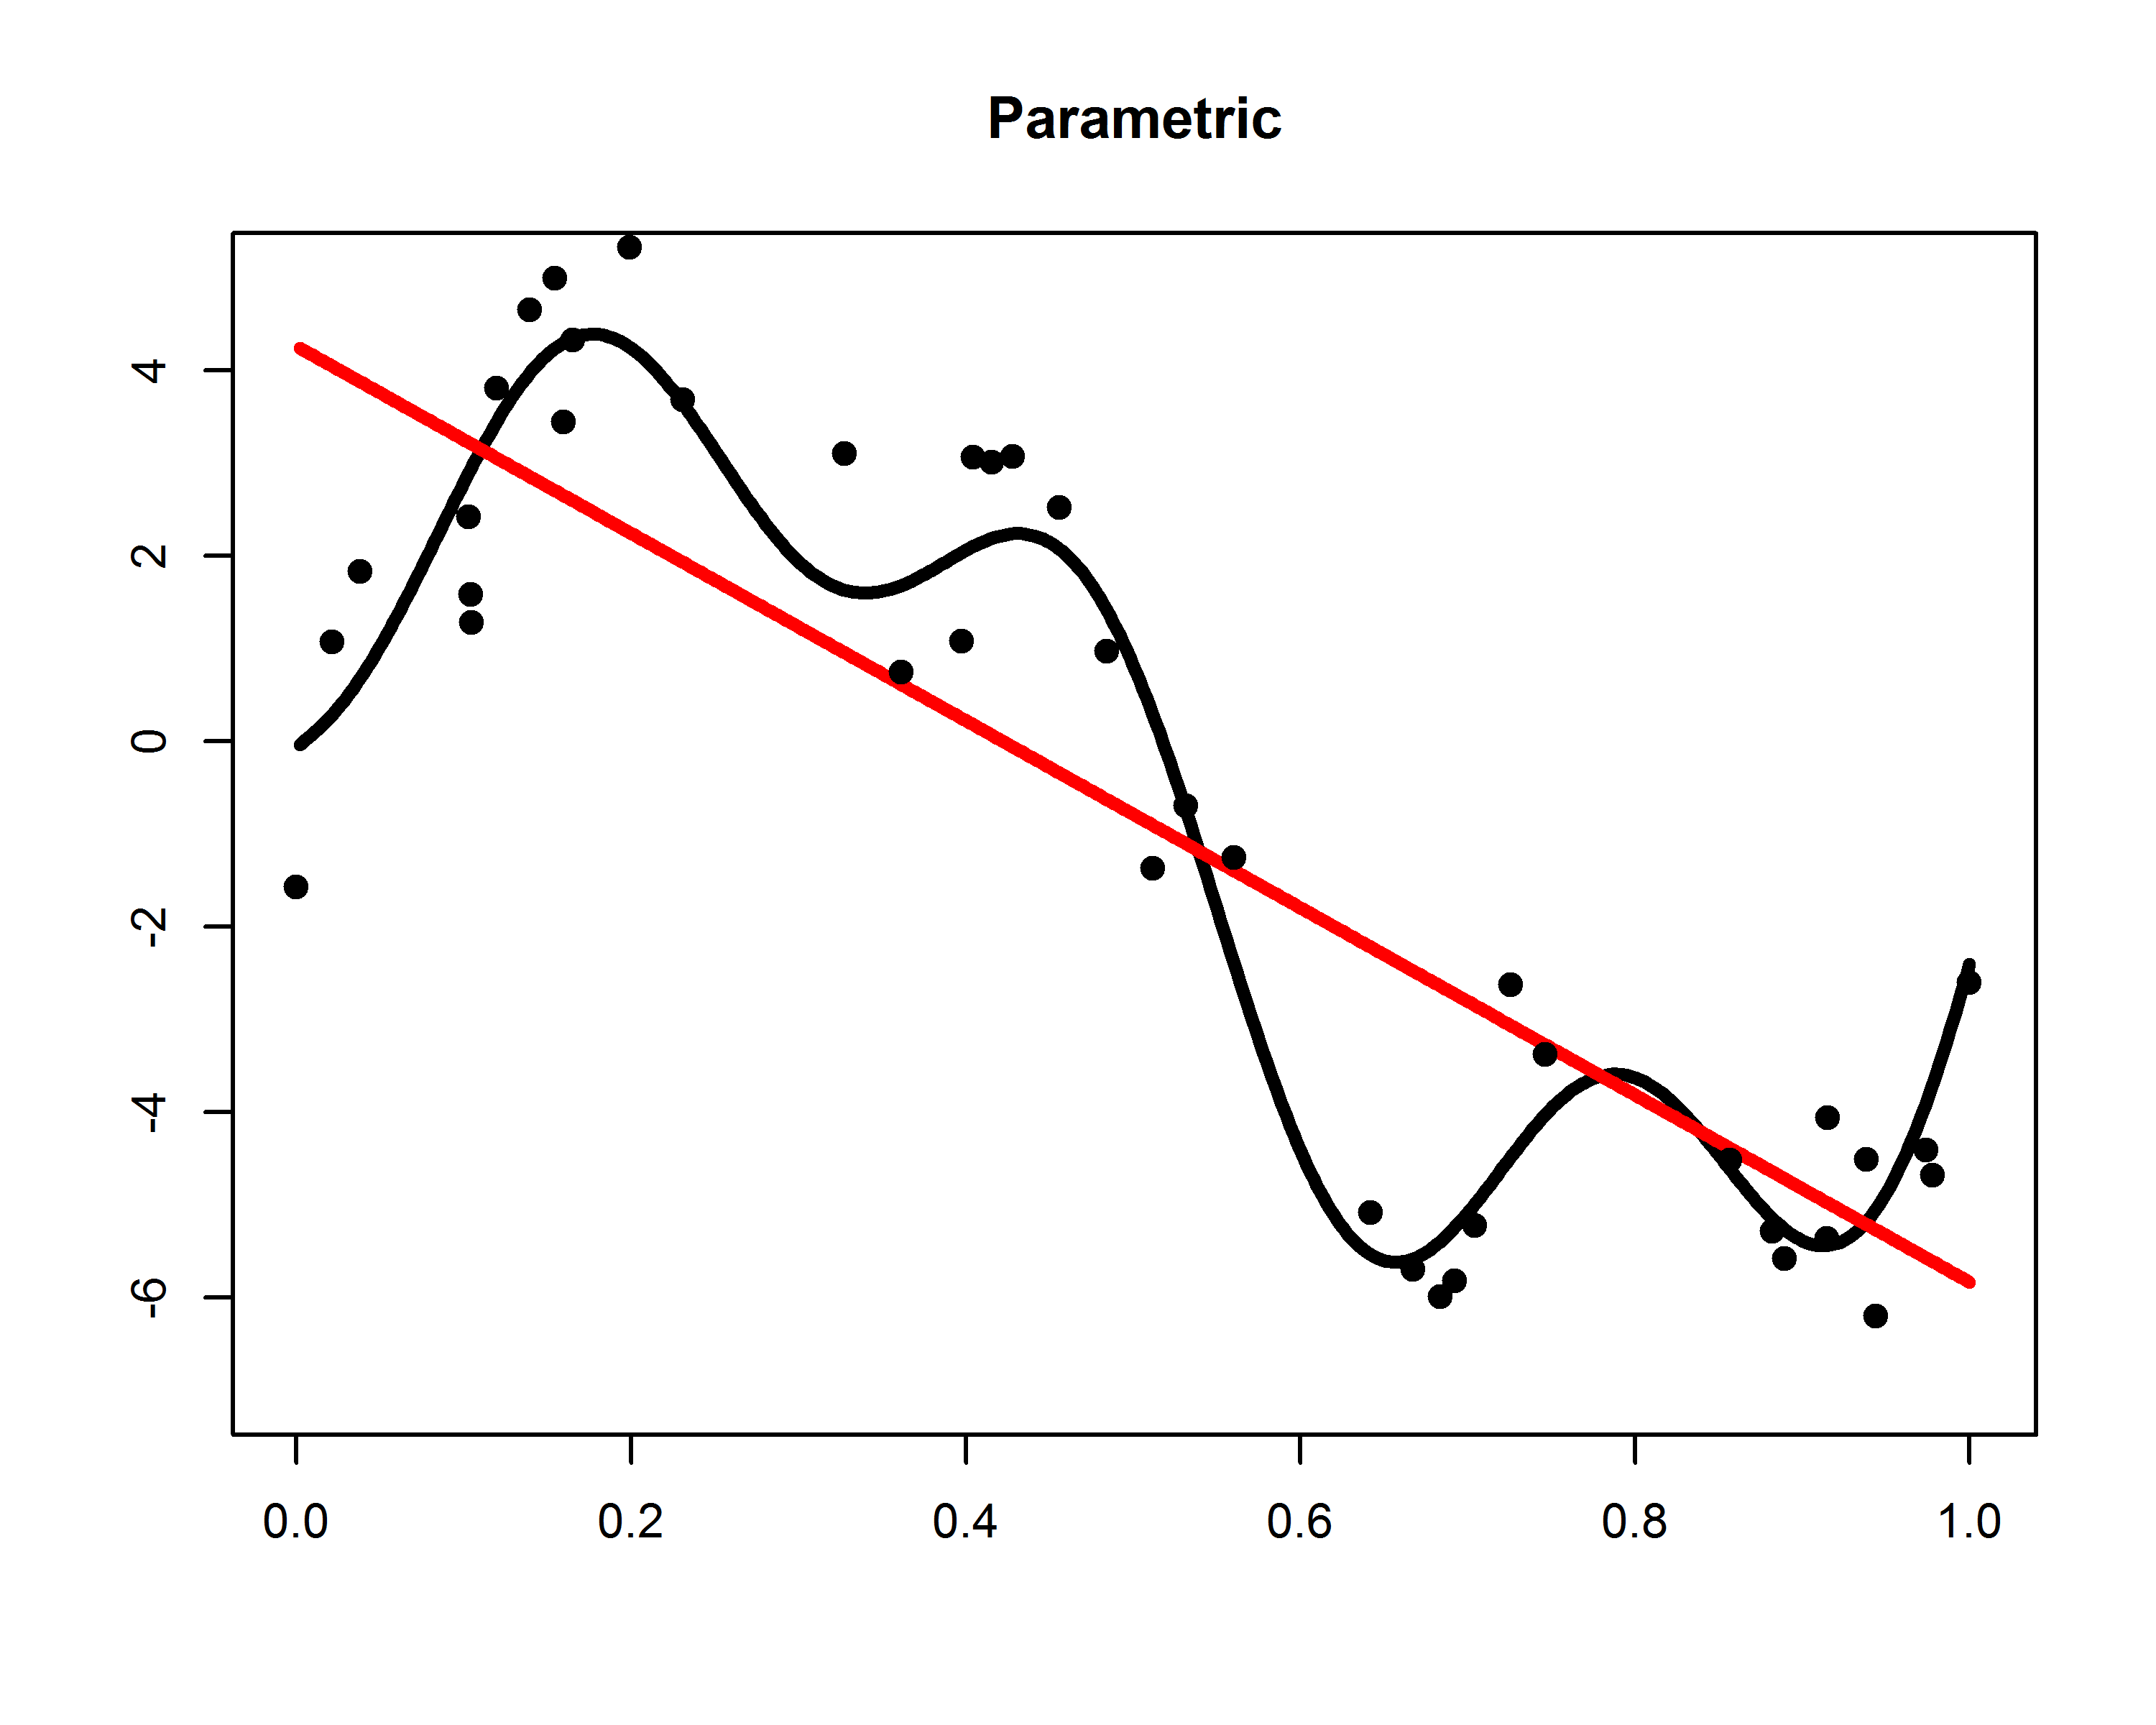
\includegraphics[width = 4in]{figures_julyan/Botond/Parametric.png}
}


\frame{\frametitle{Nonparametric fitting}
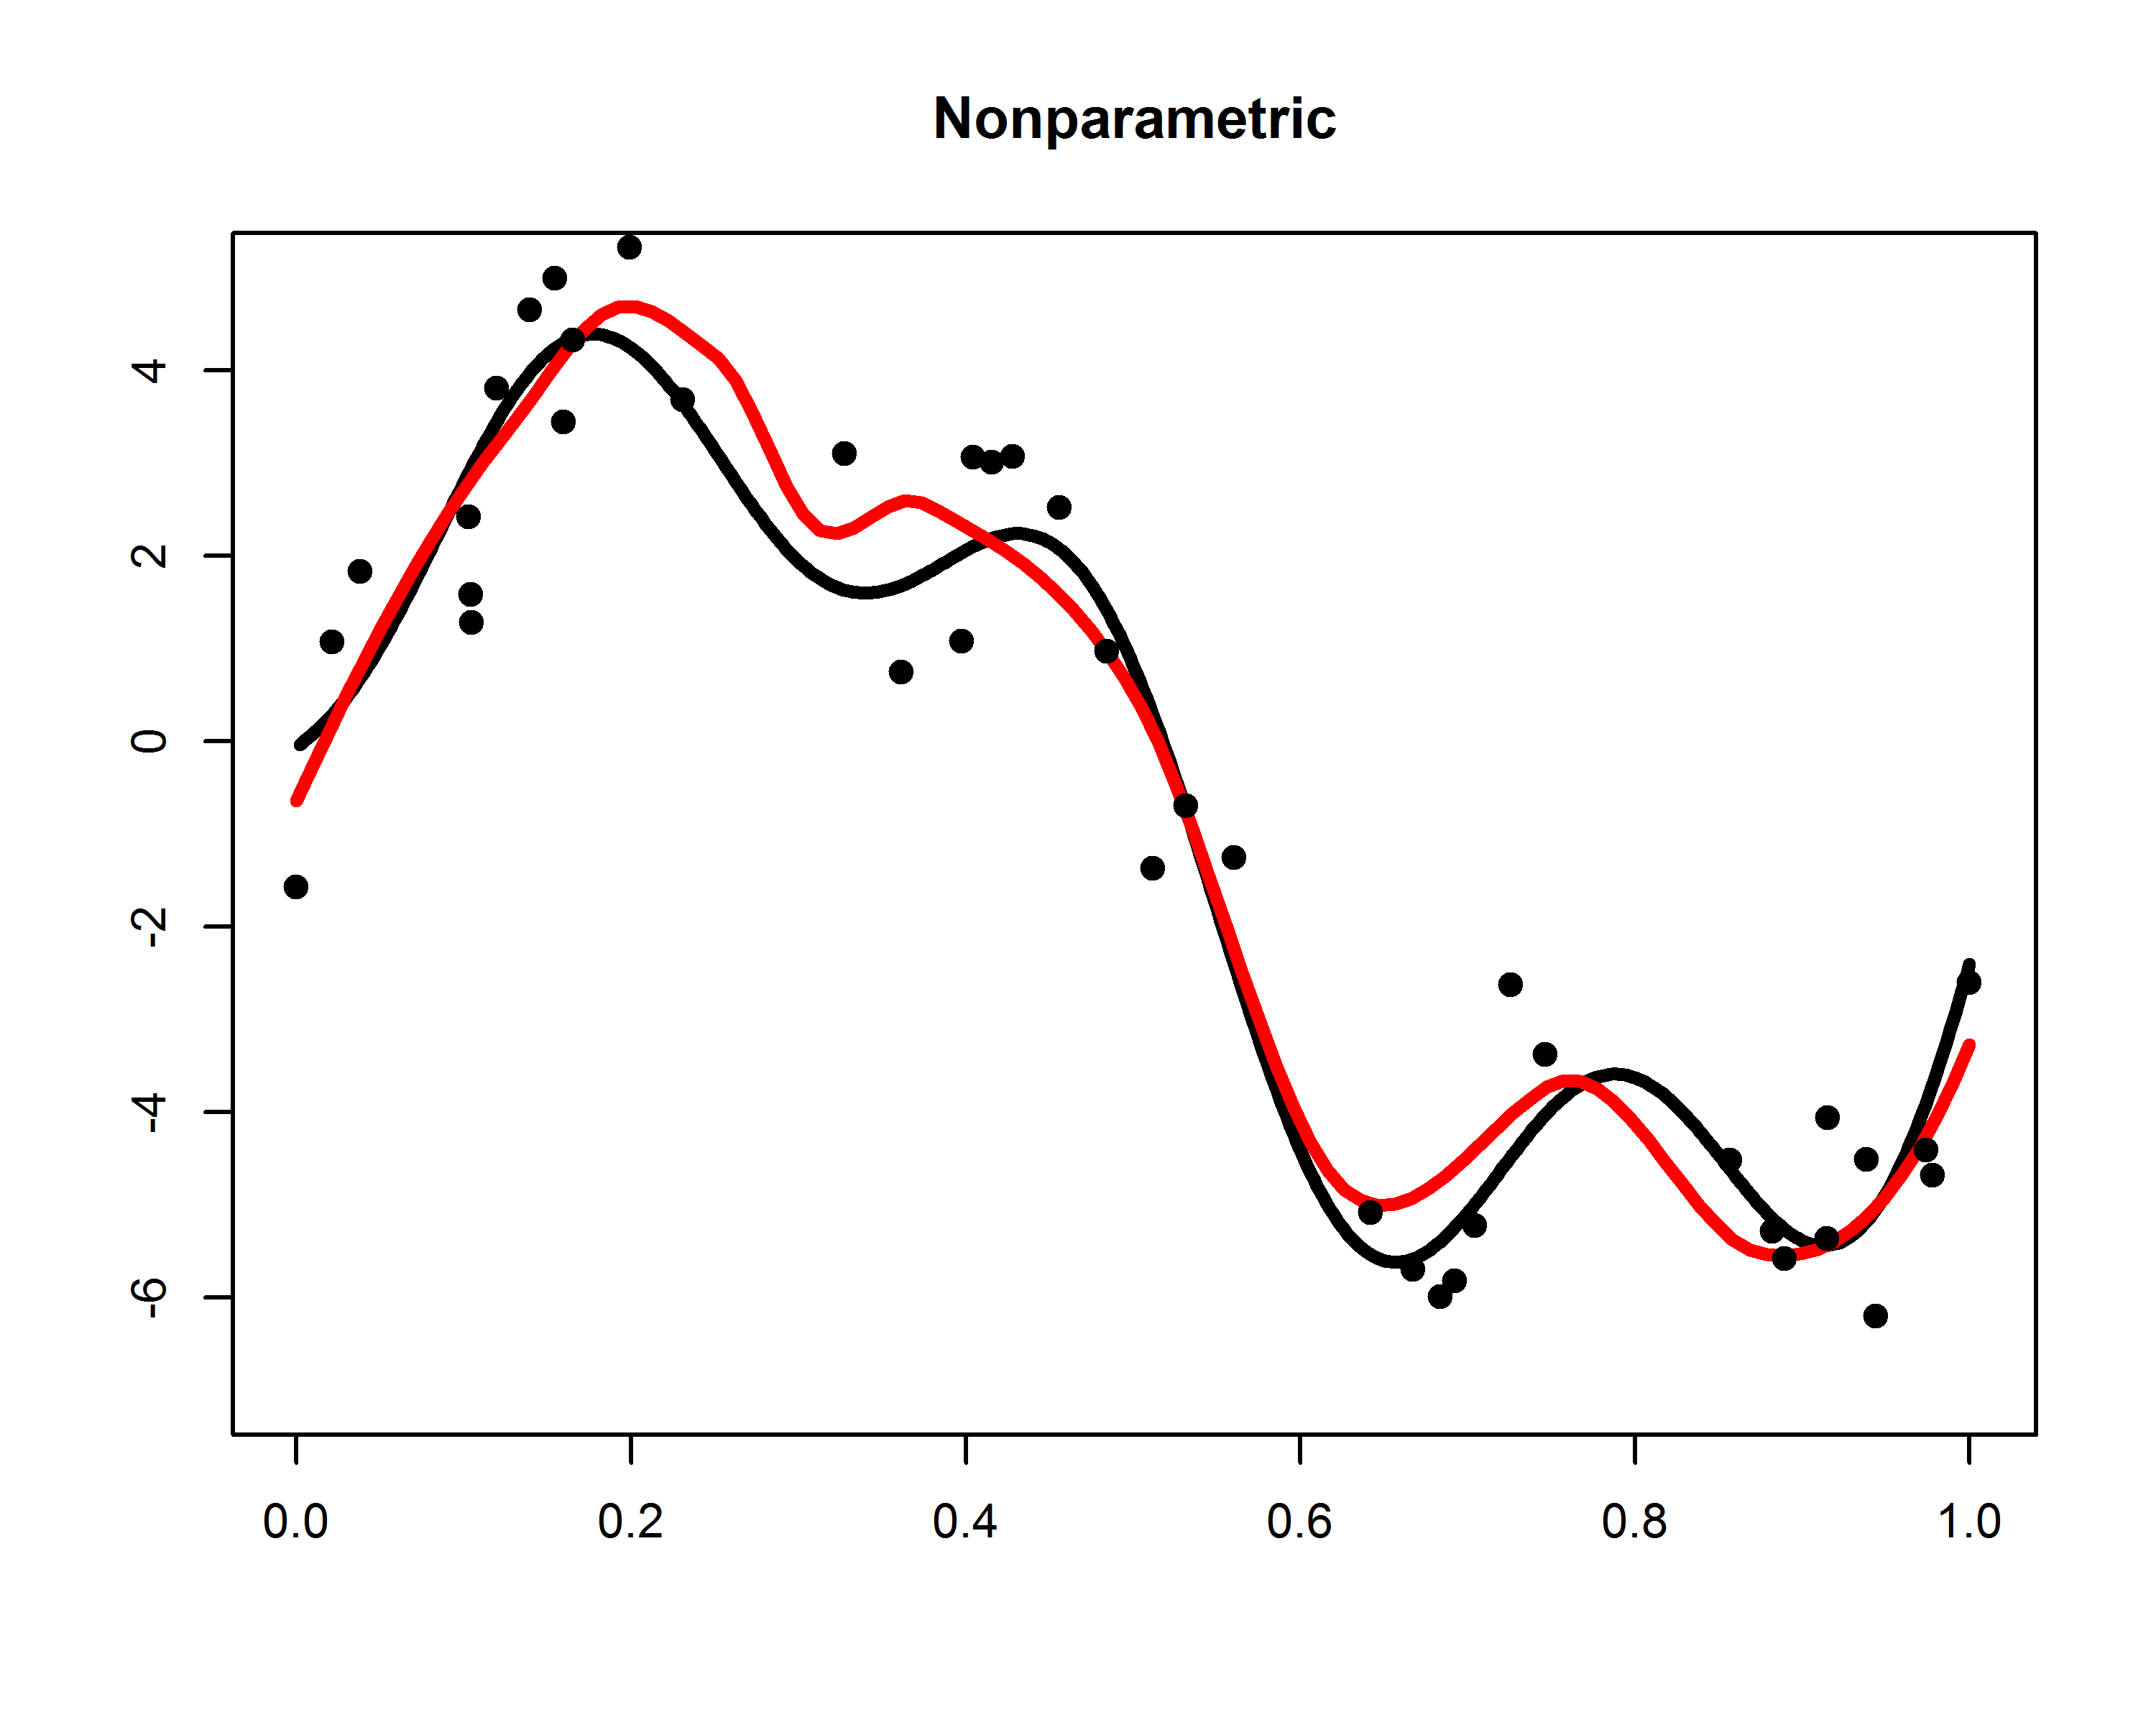
\includegraphics[width = 4in]{figures_julyan/Botond/NP.png}\vspace{-0.3cm}\\
}


\frame{\frametitle{Prior}
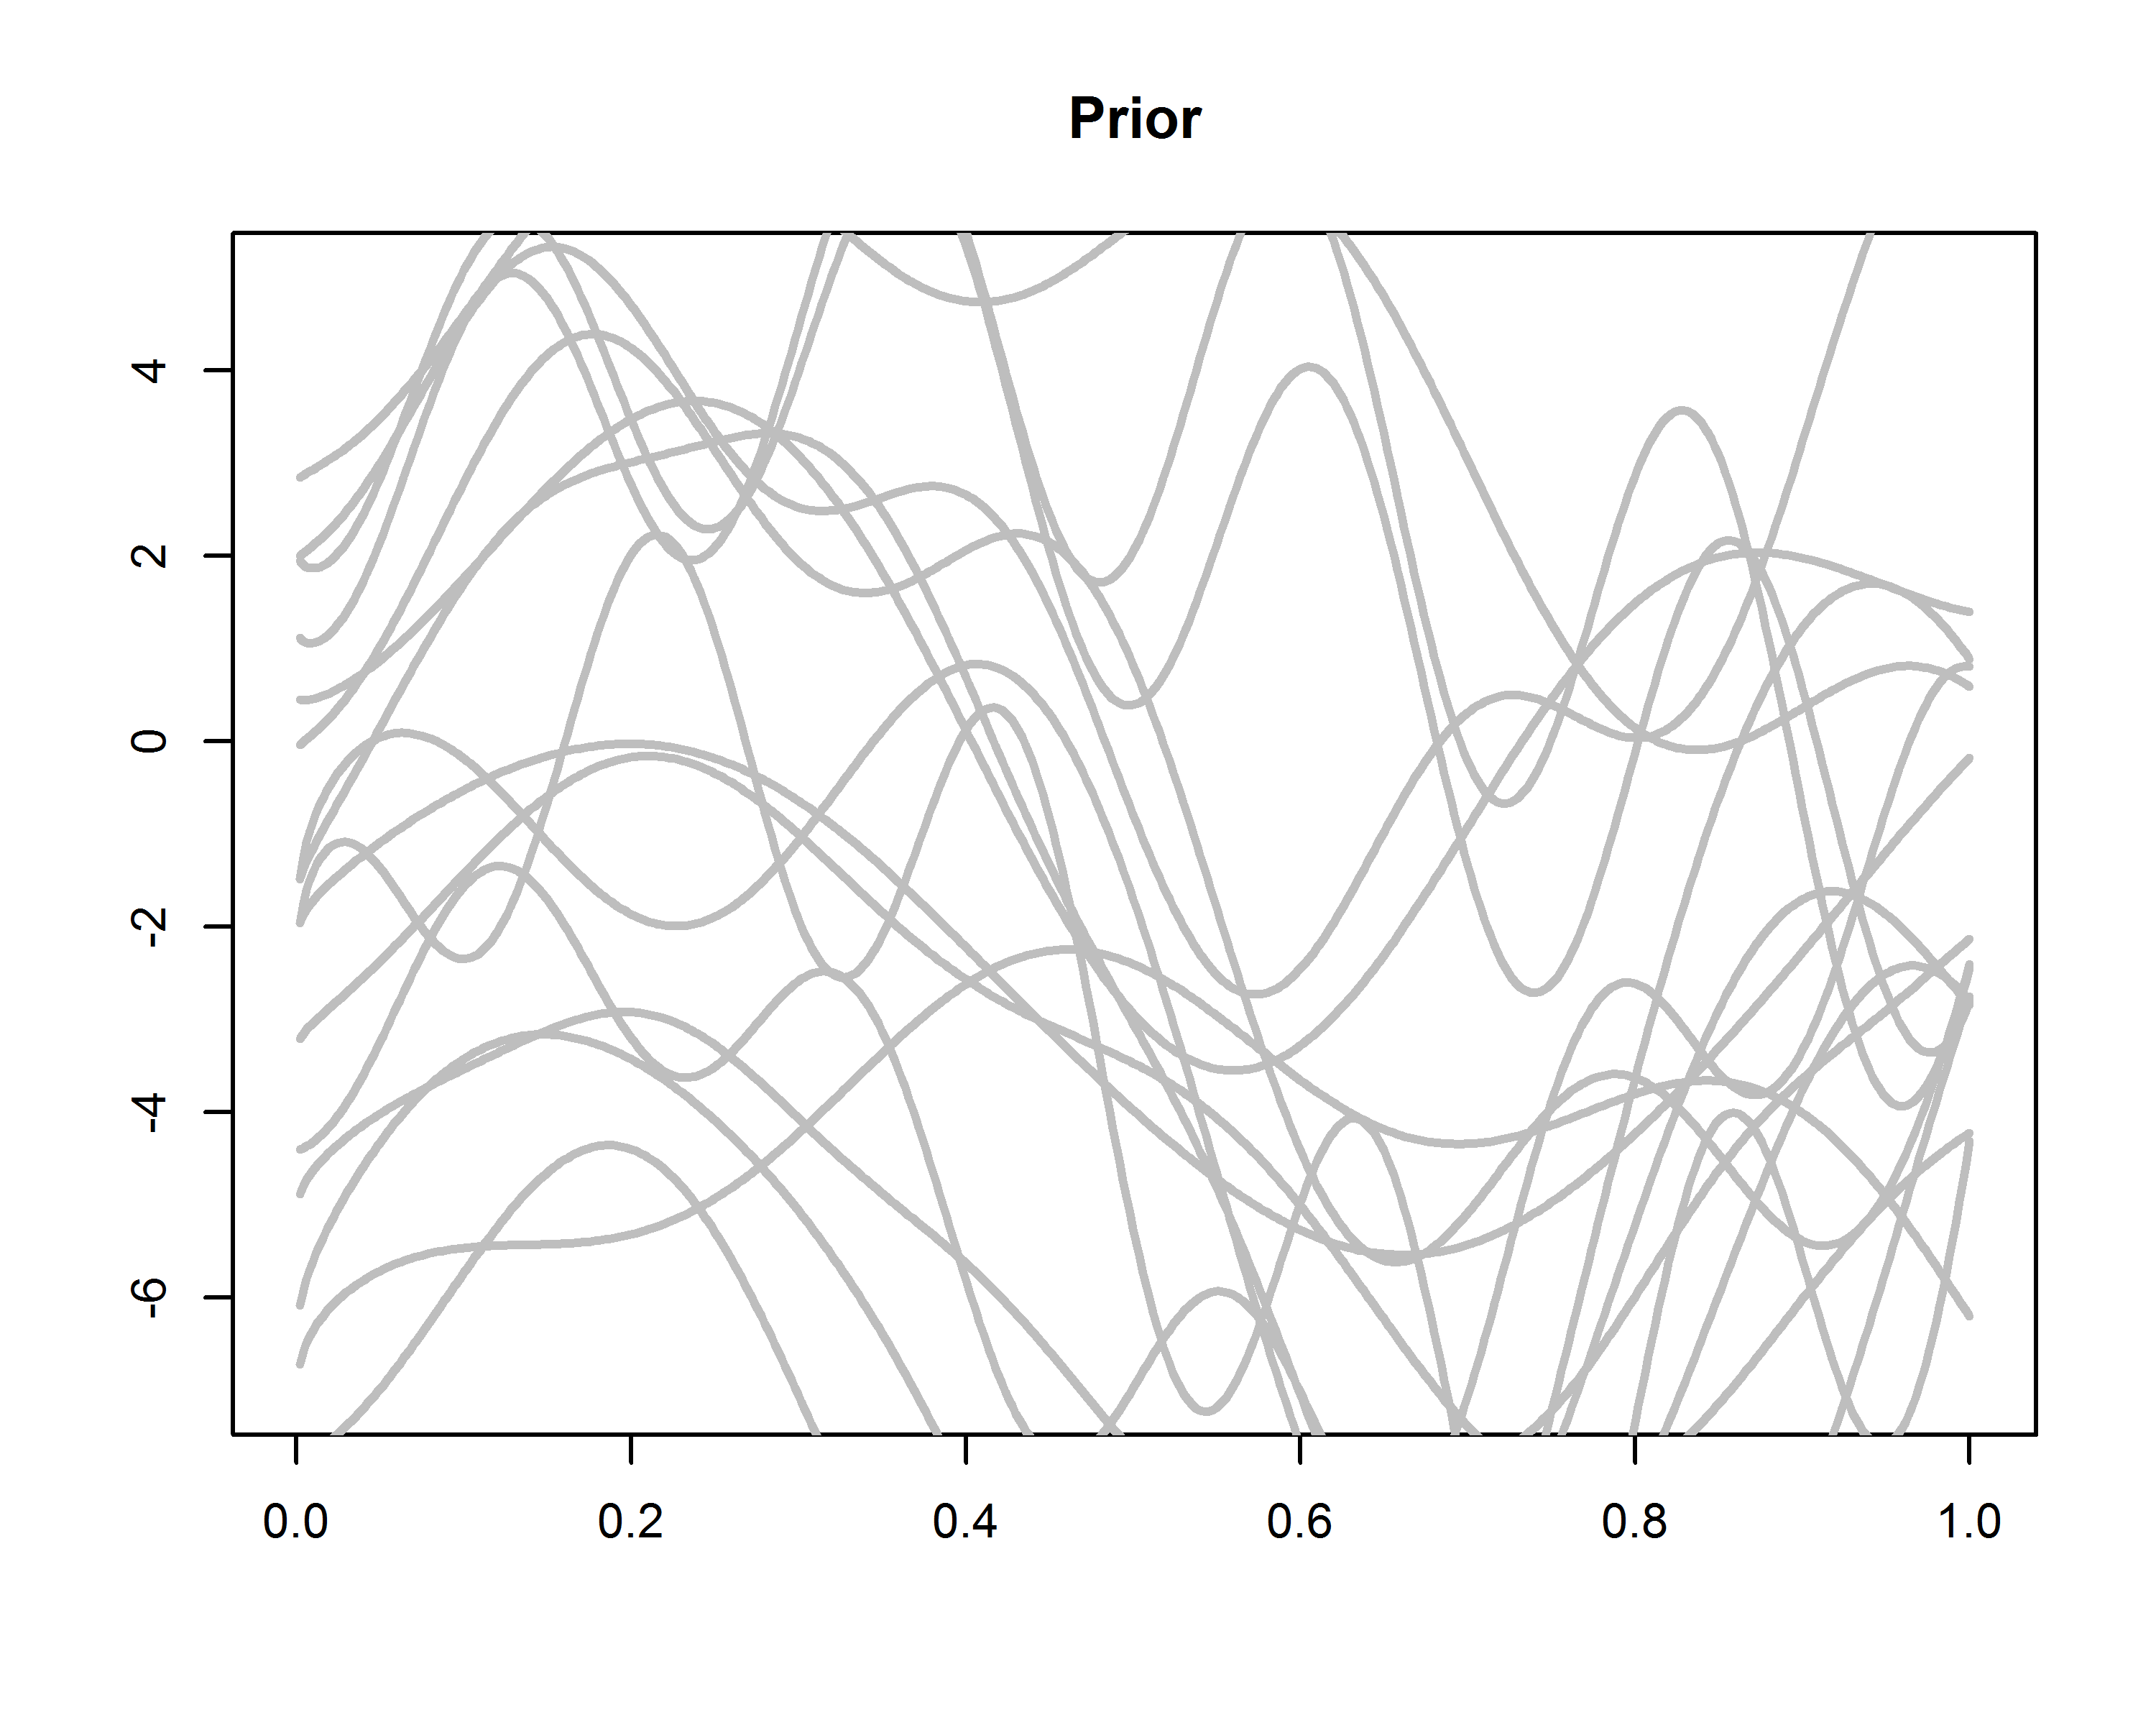
\includegraphics[width = 4in]{figures_julyan/Botond/Prior.png}\vspace{-0.3cm}\\
}


\frame{\frametitle{Posterior}
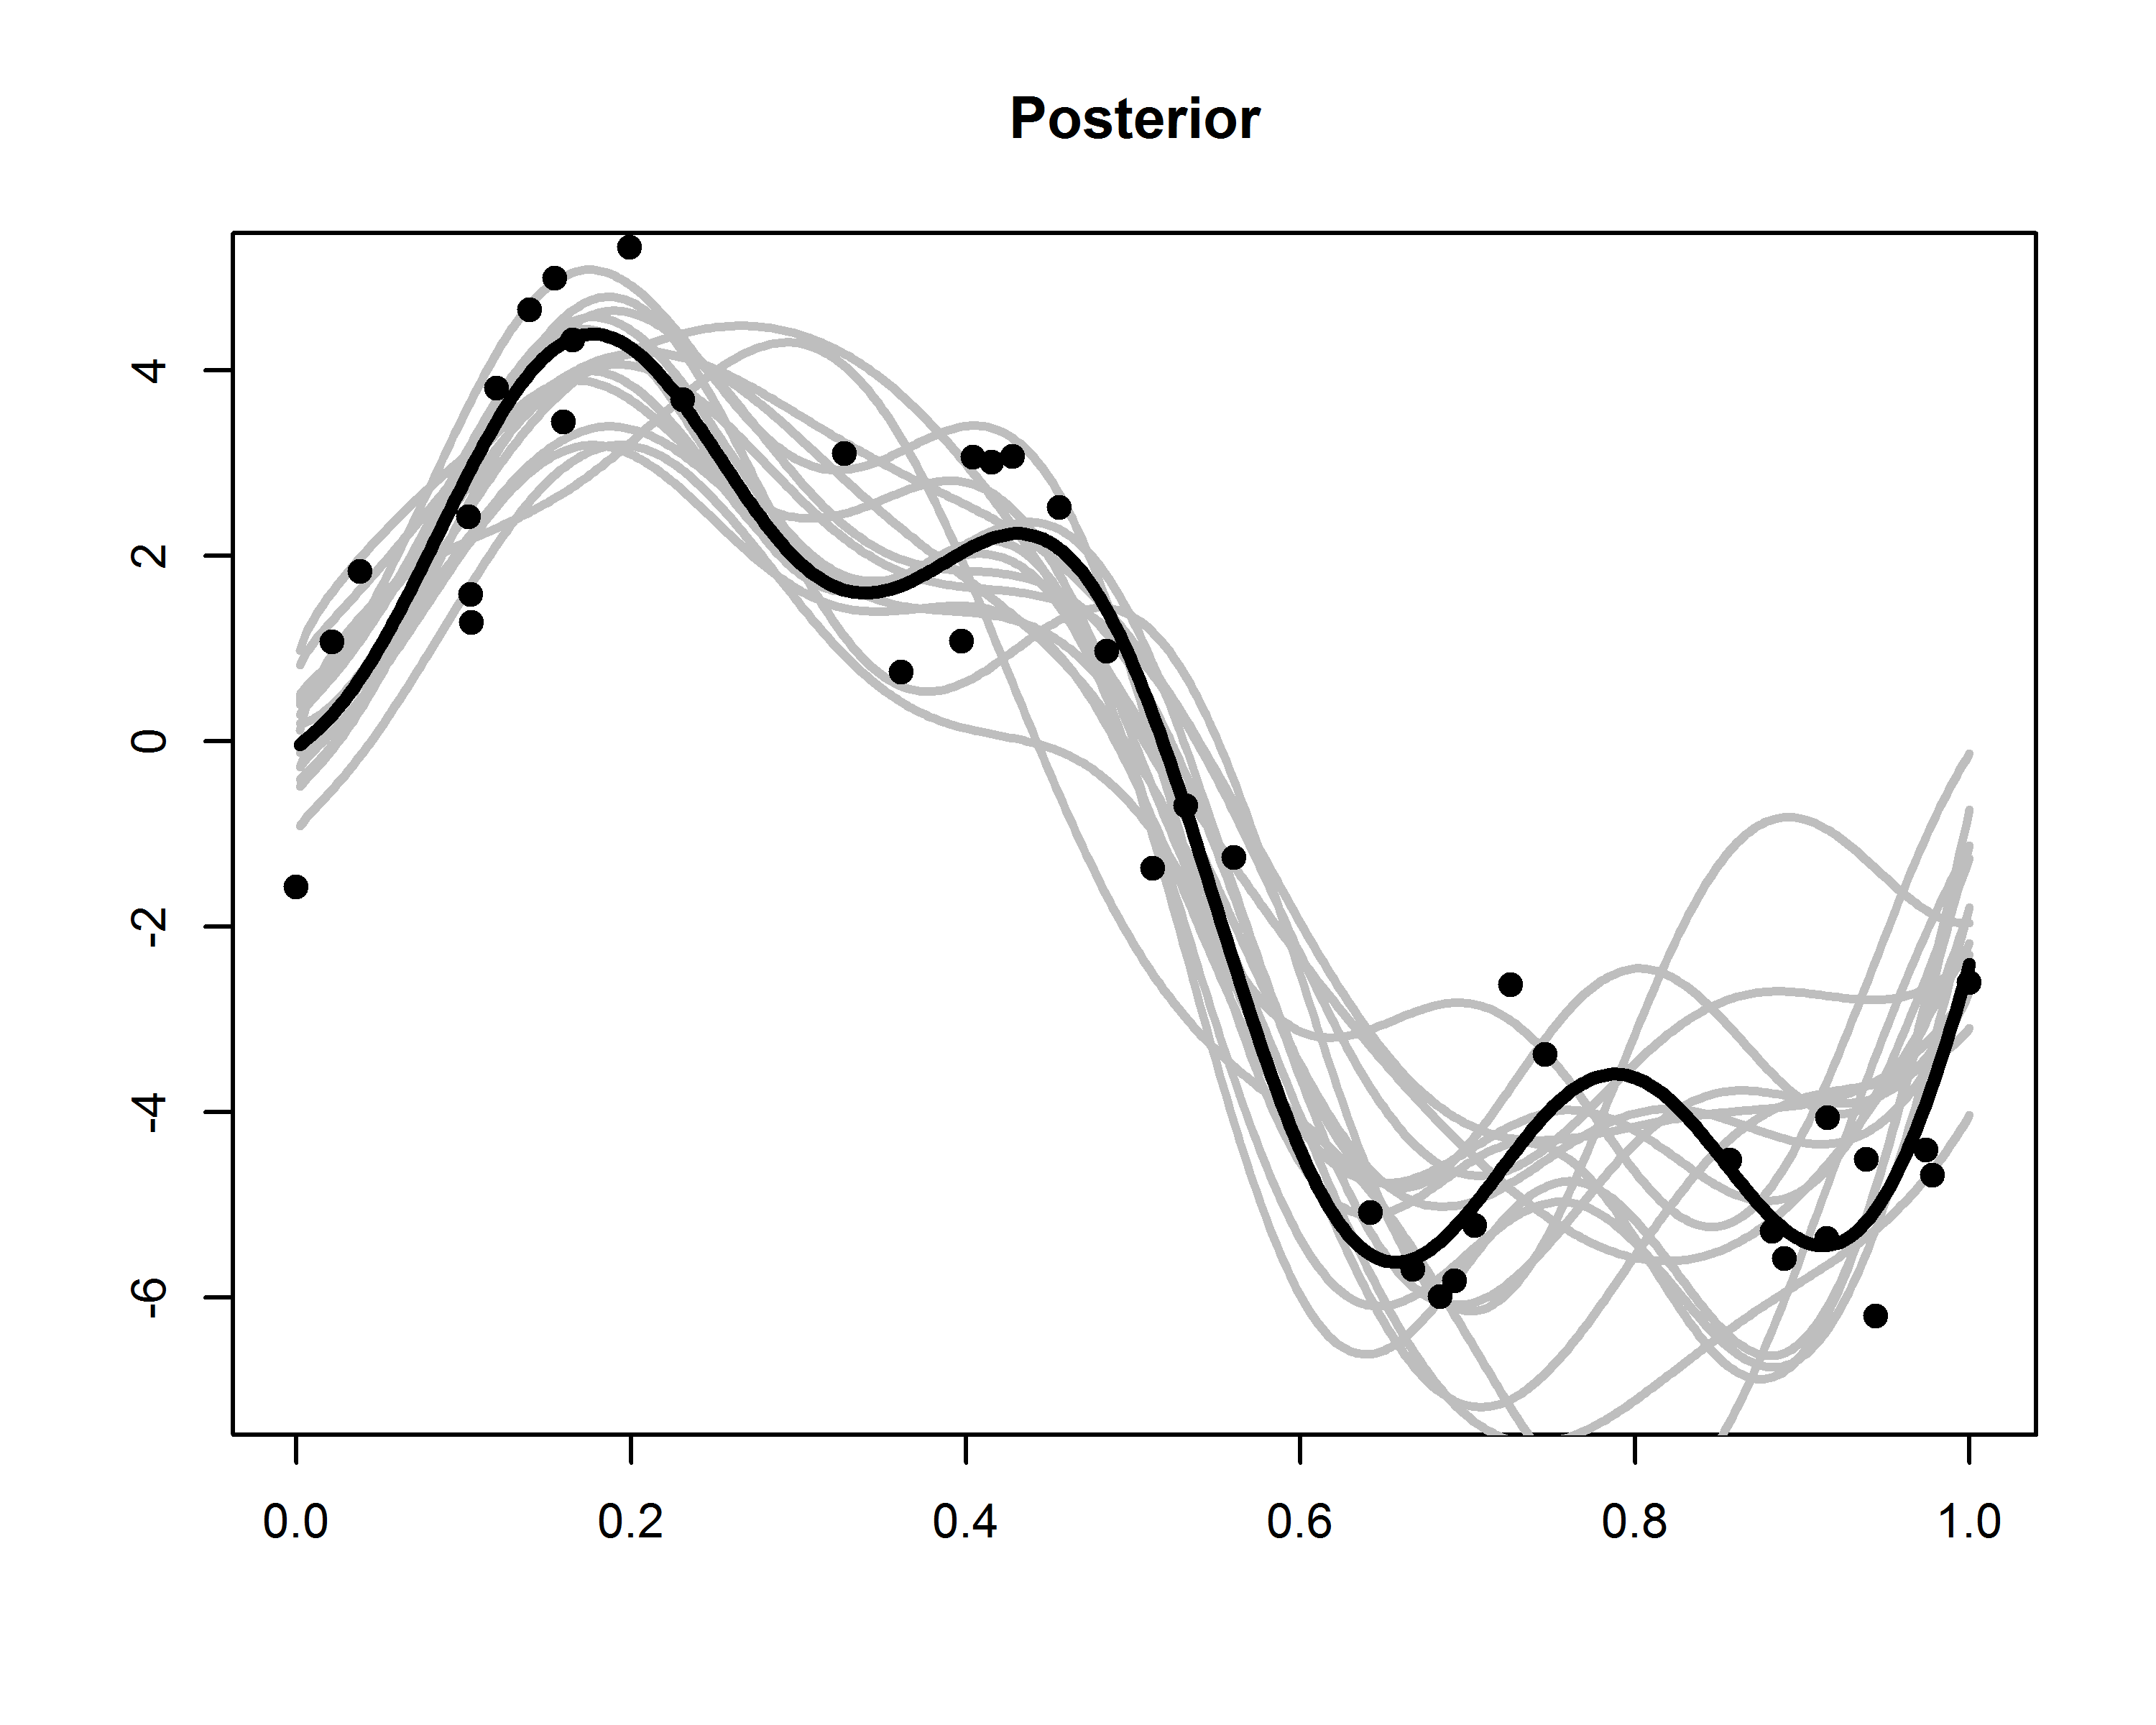
\includegraphics[width = 4in]{figures_julyan/Botond/Posterior.png}\vspace{-0.3cm}\\
}




\begin{frame}{Parametric versus nonparametric}
Complexity of the model $\{P_{\theta}:\, \theta\in\Theta\}$.\\
\vspace{-0.2cm}
\center{
\begin{tabular}{p{15mm}  p{42mm}  p{42mm}}
\toprule
Models&  \textbf{Parametric} & \textbf{Nonparametric}\\
\midrule
Dimension&  \textcolor{red}{Finite} dimensional $\Theta$ & \textcolor{red}{Infinite} dimensional $\Theta$ \\
&&\\
Pros&  \textcolor{red}{Easier} to handle and make interpretations of the results  & \textcolor{red}{Less} chance for \textcolor{red}{misspecifications } \\
& Computationally \textcolor{red}{faster } & More \textcolor{red}{flexible } \\
&&\\
Cons&  Without strong belief in the particular structure of the model \textcolor{red}{not reliable } &
\textcolor{red}{Computationally} and analytically \textcolor{red}{challenging }\\
&&\\
Examples&  \textcolor{red}{Poisson} (number of car crashes, typos in a book)  & Density, regression \textcolor{red}{function} estimation \\
& \textcolor{red}{Normal} distribution (grades of students, height, weight, footsize of people) &
\textcolor{red}{Clustering} (unknown cluster size and number)\\
\bottomrule
\end{tabular}
}
\end{frame}



%%%%%%%%%%%%%%%%%%%%%%%%%%%%%%%%%%%%%%%%%%%%%%%%%%%%%%%%%%%%%%%%%%%%%%%%%%%%%%%%%%%%%%%%%%%%%%%%%%%%%%

\frame{\frametitle{Noisy picture}
\center{

\includegraphics[width = 3.8in]{figures_julyan/Botond/Baby-Seal-Noisy3.jpg}
}}
\frame{\frametitle{Parametric}
\center{
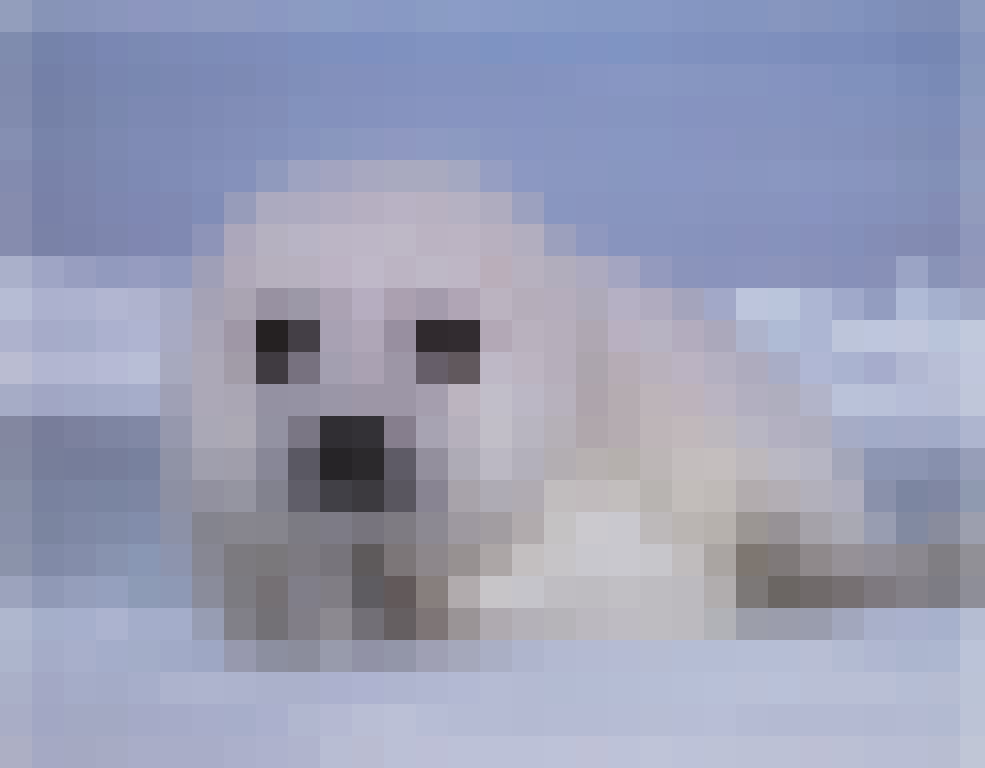
\includegraphics[width = 3.8in]{figures_julyan/Botond/Baby-Seal-LowRes2.jpg}
}}
\frame{\frametitle{Nonparametric}
\center{
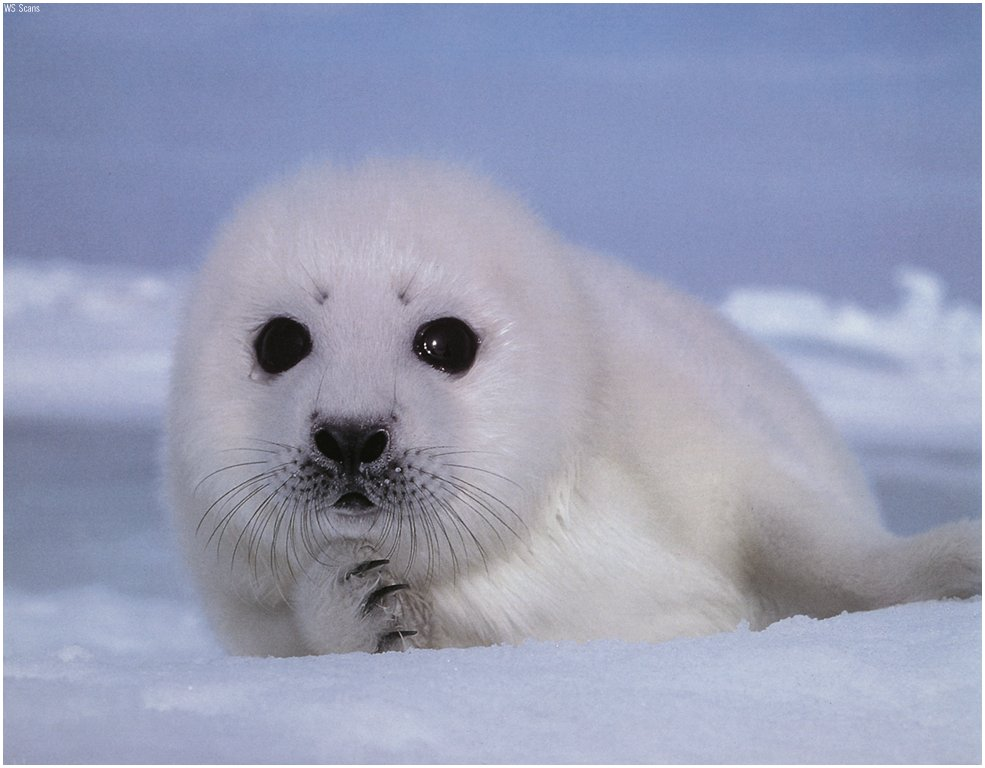
\includegraphics[width = 3.8in]{figures_julyan/Botond/Cute-Baby-Seal.jpg}
}}





\begin{frame}{Bayesian nonparametric priors}
\begin{block}{Two main categories of priors depending on parameter spaces}\medskip
\begin{columns}
\column{.4\textwidth}
%\begin{itemize}
%\item 
\visible<2->{\textcolor<2>{red2}{Spaces of functions\\\textit{random functions}}
\begin{itemize}
\item Continuous stochastic processes\\
e.g. Gaussian processes
\item Random basis expansions
\item Random densities (expon.)
%\end{itemize}
\end{itemize}}
\column{.6\textwidth}
%\begin{itemize}
%\item 
\visible<3->{\textcolor<3>{red2}{Spaces of probability measures\\\textit{random probability measures} (RPM)}
\begin{itemize}%[<+->]
\item \textcolor<4>{red2}{Often discrete proba. measures\\
Cornerstone: Dirichlet process}\\
We'll see others: Pitman--Yor, Normalized generalized gamma process, Normalized stable process, Gibbs-type processes, Normalized random measures, etc}
\end{itemize}
%\end{itemize}
\end{columns}
\end{block}
\begin{center}
\only<2>{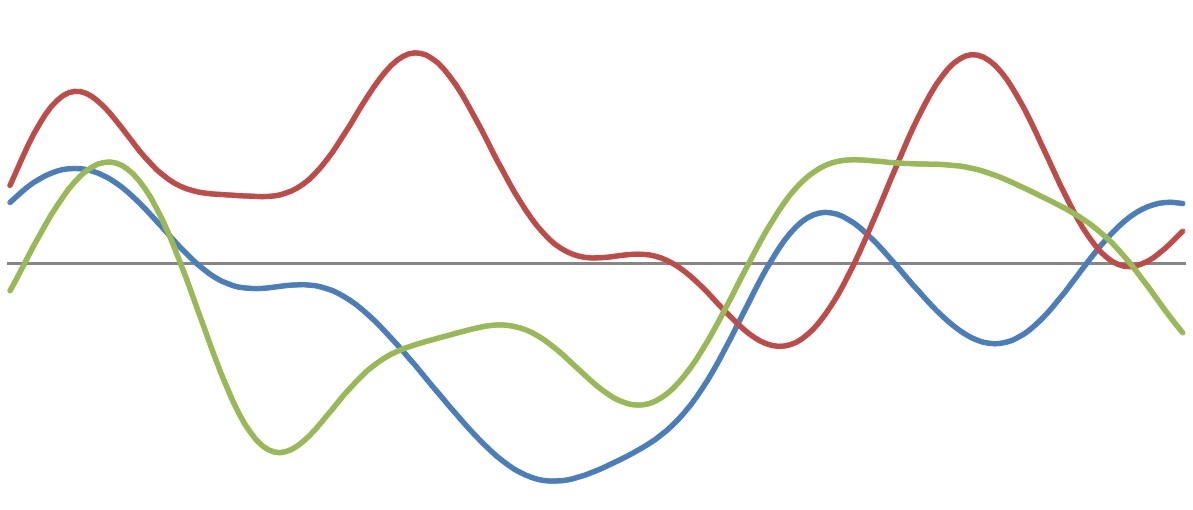
\includegraphics[width=.7\textwidth]{figures_julyan/introRPM/GPsamples}\\
\flushright[Wikipedia]}
\visible<3->{
\begin{center}
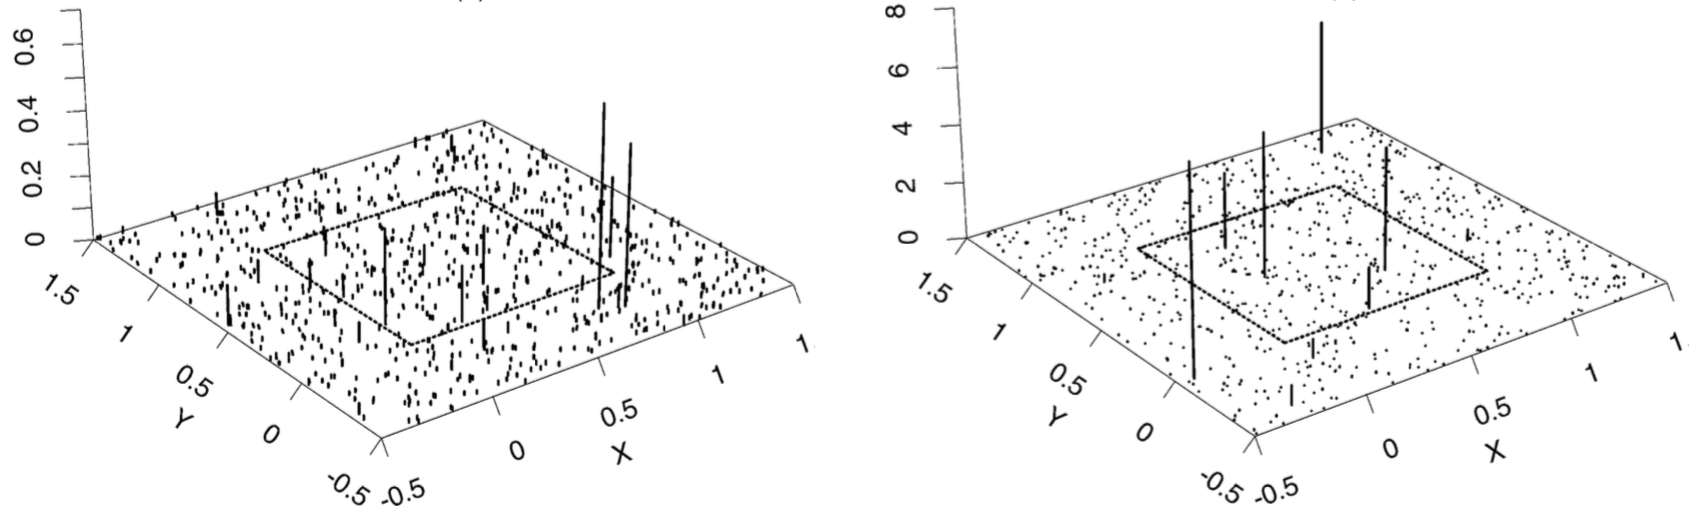
\includegraphics[width=\textwidth]{figures_julyan/introRPM/brix_draws}\\
\flushright %\textcolor{blue}
\citep{brix1999generalized}
\end{center}
}
%\visible<>{\includegraphics[width=\textwidth]{•}}
\end{center}
\end{frame}





\begin{frame}{References}
\begin{itemize}
	\item \alert{One of the first textbooks}: \fullcite{Ghosh2003}
	\item \alert{One that reads very well}: \fullcite{hjort2010bayesian}
	\item \alert{Quite a comprehensive one on the theory side}: \fullcite{ghosal2017fundamentals}
	\item \alert{Chapter 31} on Nonparametric Bayesian models of \fullcite{murphy2023probabilisticMLadvanced} (as of today, the full version of this chapter can be found in the supplementary of the book)
\end{itemize}
\end{frame}

